\section{PacketSkip Explained}
\label{sec:protocol}

For understanding the optimizations proposed in this paper it is important to understand the protocol of PacketSkip first. In this section we briefly recapitulate the basics of a Skip Graph data structure, followed by a short reminder how PacketSkip elaborates on this design. We complete this summary with a description of the internal representation of data and of the routing protocol that grants access to that data.

PacketSkip is a distributed indexing data structure derived from a Skip Graph. It works as an over-overlay to any DHT-based p2p network and provides a sorted set of index items. The index can be searched via multi-dimensional range queries. The current use case is the retrieval of peer capacities where the capacity features -- such as CPU, storage or bandwidth -- are the dimensions and the peer's contact information is the actual search object. However, PacketSkip is not limited to this use case or to a predefined set of dimensions. It is already possible to index e.g. multimedia data files in PacketSkip and associate their meta data with a certain peer offering them.

The main interface to PacketSkip is a service running on each peer. The service provides access to the index's update and search mechanisms. Also, the service maintains the nodes of the underlying distributed Skip Graph where the data is actually stored. In short: it manages the inter-PacketSkip communication as well as the communication to PacketSkip from the outside. For applications which use the service to store and retrieve index items, the inner workings of PacketSkip are basically a black box. The system itself does not care about the use case of the data. For our purposes we implemented a capacity manager application that stores periodically peer capacities and queries them on demand.

\subsection{Skip Graphs}
\label{subsec:skipgraph}

A Skip Graph is a distributed data structure with logarithmic access times on average. It uses a probabilistic approach to establish edges between its nodes. Nodes in a Skip Graph have no global knowledge and there is no hierarchical differentiation between nodes. The nodes are responsible for a certain range in the feature space and sorted in the graph via this responsibility. The feature space is completely and disjointly divided by the nodes.

Skip graph nodes are linked to other nodes on several doubly linked lists with head and tail of each list also linked -- each one effectively forming a ring. The rings are assigned to different levels. On level 0 all nodes are strung in one global ring. Then recursively: a ring on level $i$, $i \in \{0,\dots,l\}$ and $l$ the currently highest level, is split in two disjoint subsets forming two new rings on level $i+1$. The ordering in the rings is kept intact. The allocation of nodes to rings is done locally when a node joins the graph. While every node is member of the only ring on level 0, for each higher level it choses randomly a sample $s \in \{0, 1\}$ and joins the ring associated to $s$ by connecting with its predecessor and successor (in respect to the ordering). The recursion ends when a node is the only node in a ring on its highest level. In summary: with each new level the number of rings doubles and the distance of the edges between two nodes also doubles (on average) which results in logarithmic access times.

Figure~\ref{fig:skipgraph} shows a schematic Skip Graph with 8 nodes (A,\dots,H) from left to right and the disjoint rings on its three lowest levels (0,\dots,2) from top to bottom.

\begin{figure}[htbp]
	\centering
	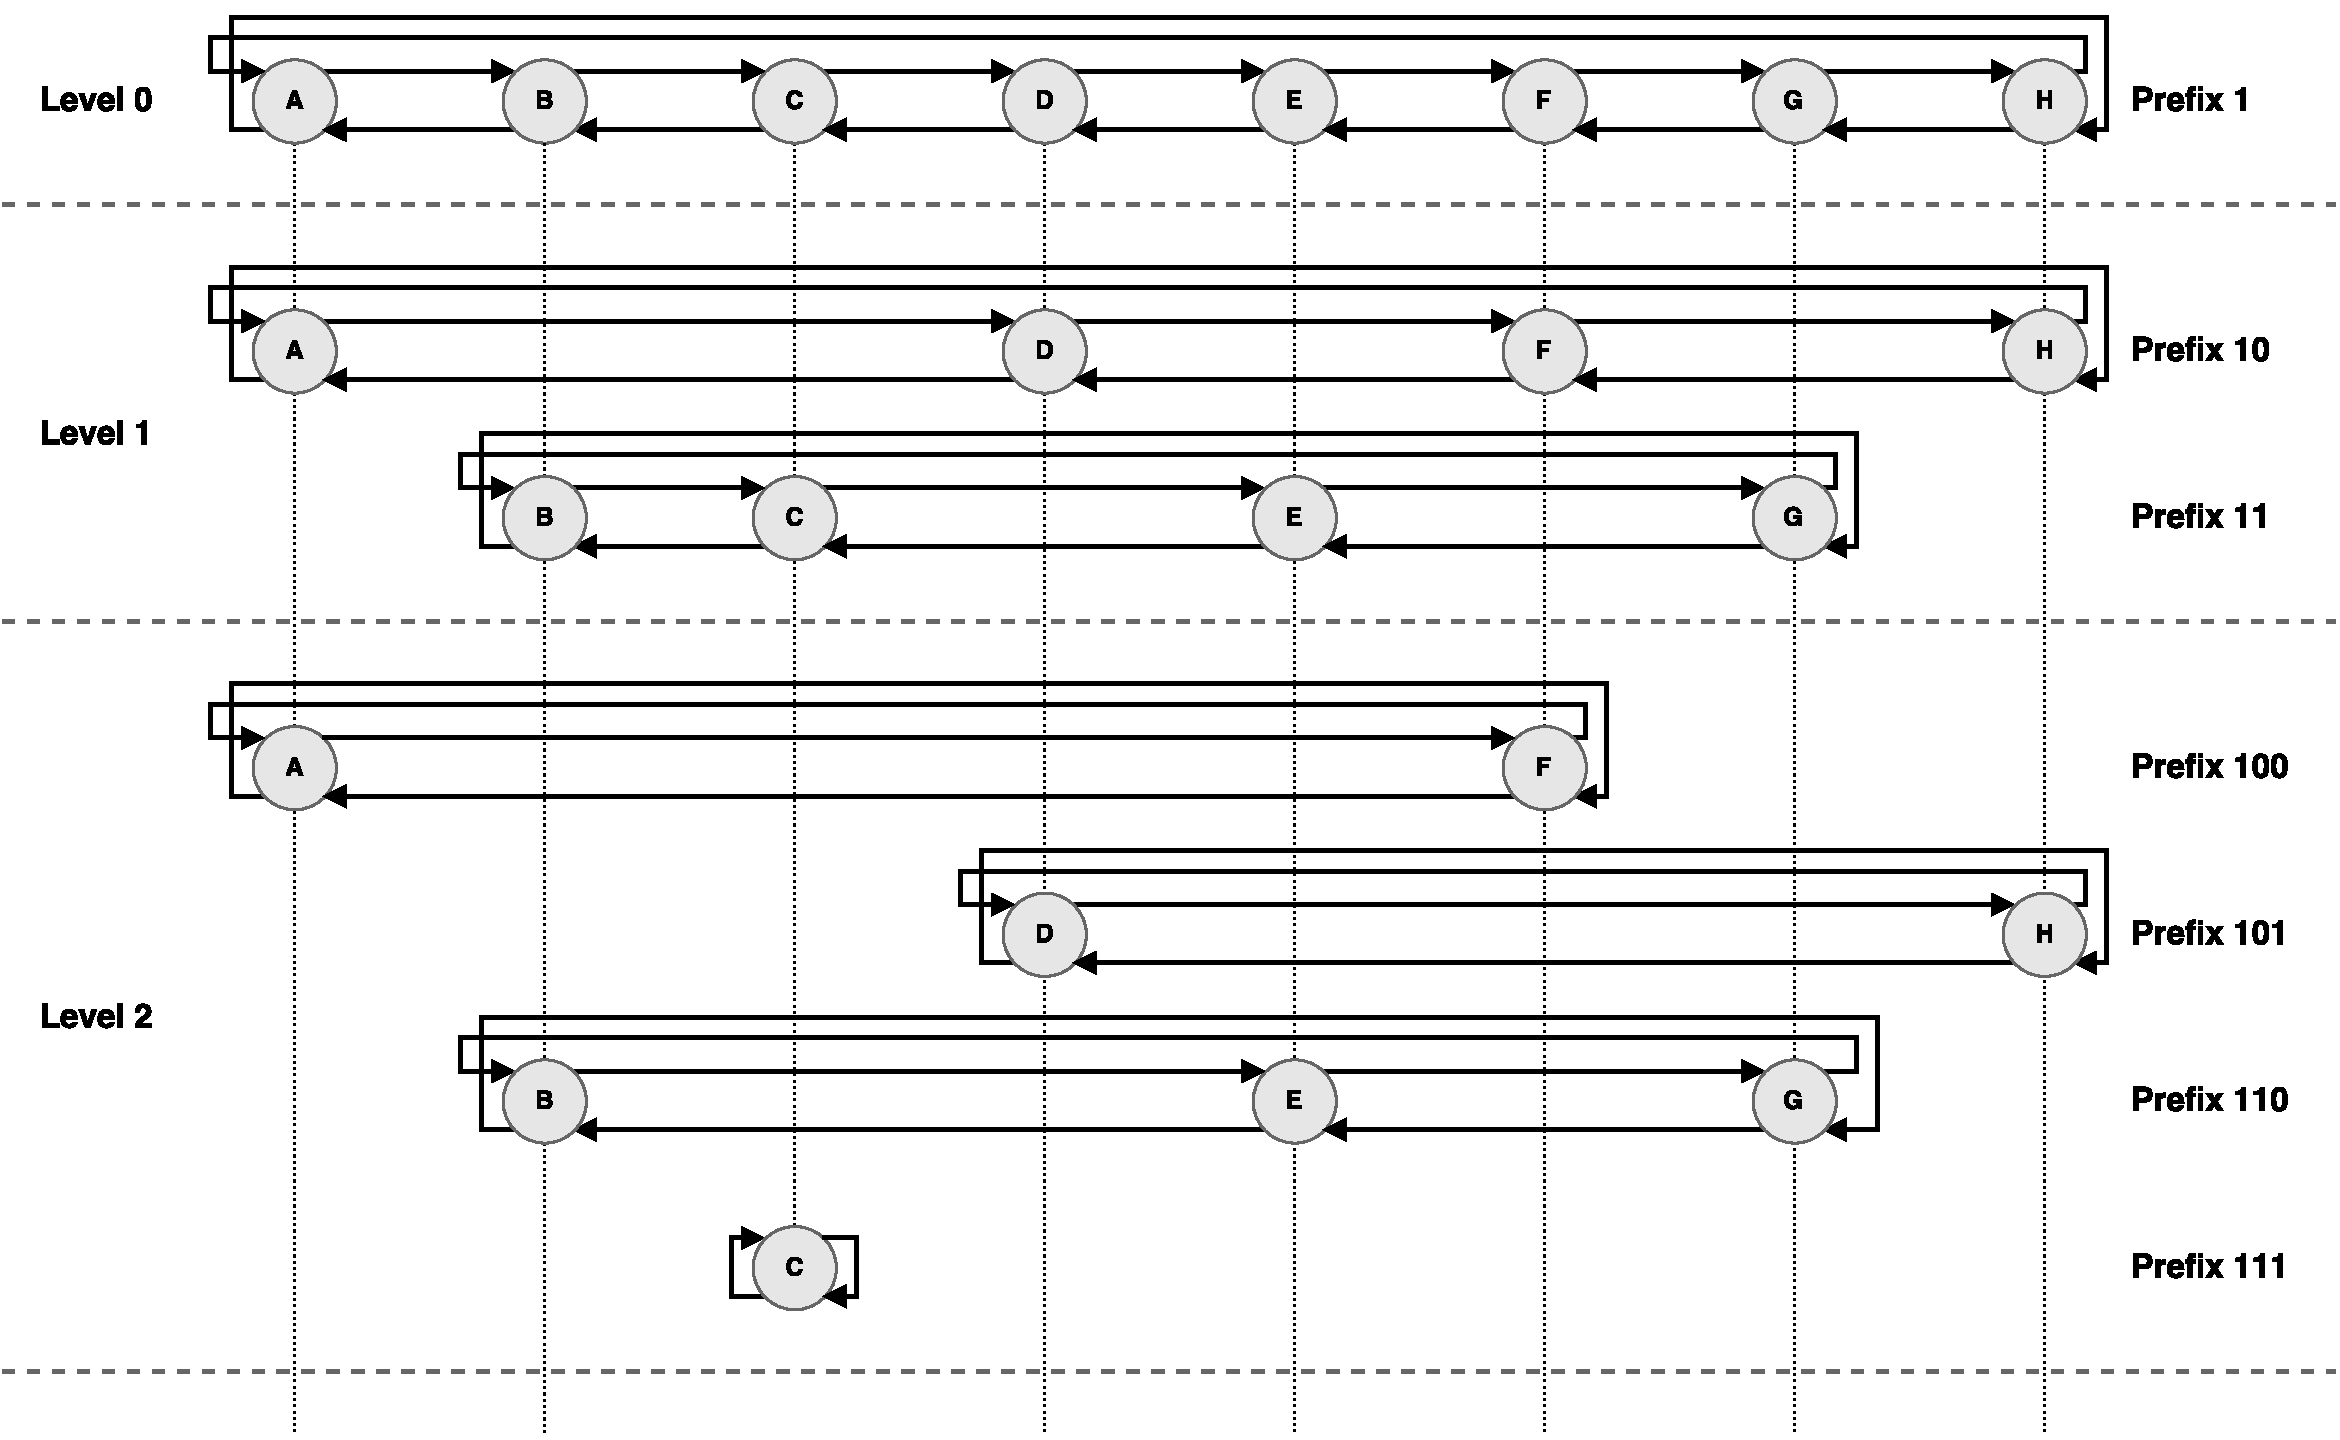
\includegraphics[width=1\linewidth]{graphics/skipgraph}
	\caption{An exemplary Skip Graph}
	\label{fig:skipgraph}
\end{figure}

\subsection{PacketSkip principles}
\label{subsec:packetskip}

The Skip Graph implementation of PacketSkip has little costs in building the graph structure. It is fully reactive and changes the graph structure only regional when nodes join or leave the graph. The join is initiated whenever a node holds too many index items and a leave operation will be performed when a node has too little items. This ensures a good load balancing. The graph will grow linearly with the number of items.

PacketSkip nodes are virtual nodes which reside on a randomly chosen peer. They are DHT objects with a fixed node id out of the overlay's id space. In the default protocol the communication between nodes is fully transparent. Messages to other nodes are addressed to their node ids. Therefore, the underlying overlay has to lookup the peer responsible for a node id with each message delivery. This ensures reliable access in dynamic systems, but it is also costly in terms of time and traffic.

Peers can host a few or no PacketSkip nodes at all. The choice of a random assignment of (PacketSkip) nodes to peers is due to the volatile and random nature of a p2p network under churn. Fixed assignments are almost impossible and load balancing re-assignments would require that node ids must be changed frequently, thereby destabilizing the PacketSkip graph as routing tables had to be updated constantly.

\begin{figure*}[t]
	\centering
	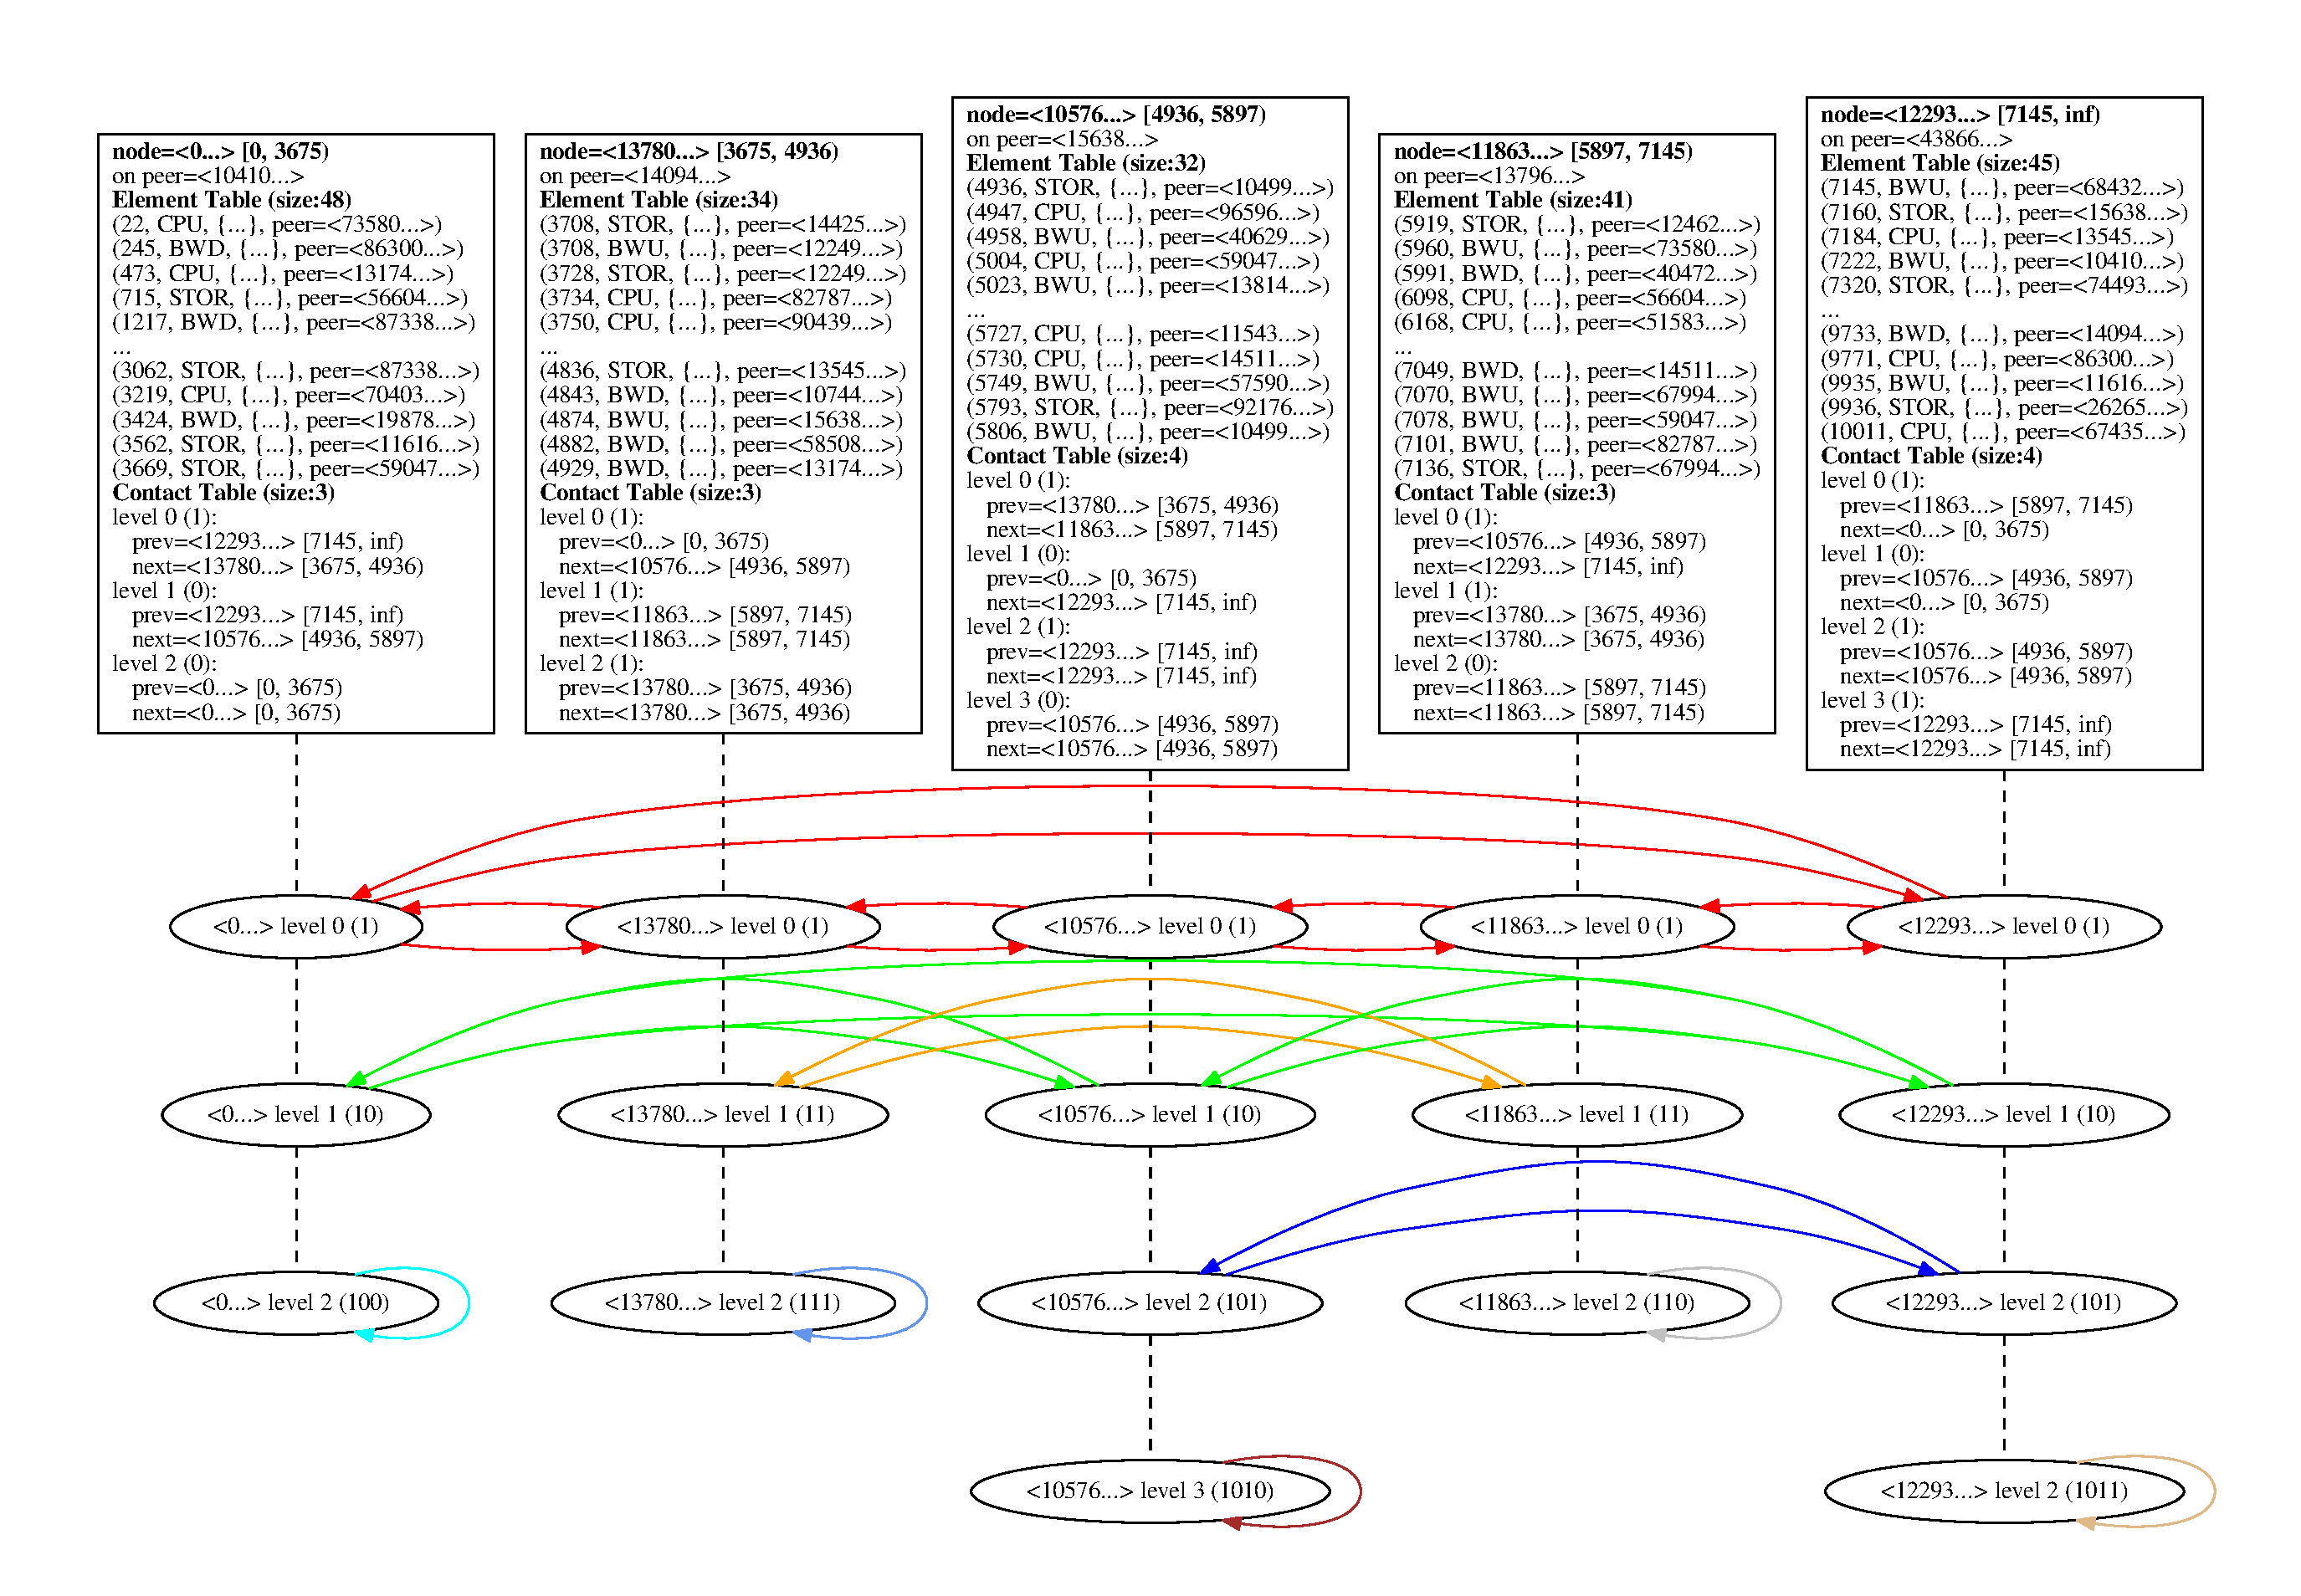
\includegraphics[width=\textwidth]{graphics/packetskipgraph_reduced}%
	\vspace{-0.3cm}
	\caption{An actual small PacketSkip graph. Illustration by Disterh{\"o}ft et al.: PacketSkip~\cite{packetskip10}}
	\label{fig:packetskipgraph}
	\vspace{-0.3cm}
\end{figure*}

Figure~\ref{fig:packetskipgraph} shows an exemplary PacketSkip graph with five nodes. Each node stores index information in an element table and pointers to its neighbors in a routing table. Pointers are visualized as edges in the graph, associated with certain levels in the underlying Skip Graph.

\subsection{Multidimensional data representation}
\label{subsec:datarepresentation}

The full capacity of a peer is described by a set of key-value pair features, for example
$\{CPU\text{:}2400,\;STOR\text{:}9583,\;MEM\text{:}123,\;BW\text{:}5000\}$. 
Whether the values are either precise measures of the given hardware or a mapping to a score is of no concern to PacketSkip as long as the usage is consistent.

In the first design of PacketSkip (v0.9) these features were plainly transformed to index items, which we call PacketSkip elements. These elements are tuples in the form: 
$(\langle key\text{=}feature\text{-}value\rangle,\;\langle feature\text{-}id\rangle,\;\langle peer | host\text{-}id\rangle)$. 
The example above results in four elements:
\begin{equation*}
\begin{split}
(2400,\;CPU, \;peer\text{=}x | ip(x)\text{:}port(x)) \\
(9583,\;STOR,\;peer\text{=}x | ip(x)\text{:}port(x)) \\
(123, \;MEM, \;peer\text{=}x | ip(x)\text{:}port(x)) \\
(5000,\;BW,  \;peer\text{=}x | ip(x)\text{:}port(x))
\end{split}
\end{equation*}

\subsection{Update and search protocol}
\label{subsec:updateandsearch}

A peer announces its capacity information to a random PacketSkip node. The node will then greedily forward the elements to its contacts according to their responsibility ranges, i.e. sending each element to the contact whose responsibility range is closest to the elements key. An element will eventually be stored in the element table of the responsible node. Feature ids are irrelevant for the distribution of elements. All features share the same one-dimensional feature space. Feature id and peer id guarantee the uniqueness of elements.

Each element is tagged with a timestamp. To avoid keeping non-active members, especially under churn, elements will be pruned after a certain time. Therefore, peers must update their capacity information on a regular basis. They may also propagate deletions of obsolete values when a capacity feature has changed, to increase search accuracy. Deletions are distributed exactly as insertions of updated values.

To establish a multidimensional search peers can formulate individual range queries for a set of capacity features. 
A search can be formulated like 
$\{CPU\text{:}[999,2730],\;STOR\text{:}[5000,6000],\;BW\text{:}[5000,\infty)\}$.
These queries are sent to a random PacketSkip node. In the original design the node will split each range queries according to the responsibilities of its contacts and forward them just as updates via a divide and conquer approach. While PacketSkip elements are one-dimensional points in the feature space, search queries are one-dimensional ranges in the same features space. So, distributing range queries inside PacketSkip used to be costly in v0.9 since many nodes could be involved. Also, as PacketSkip elements were one-dimensional, the multidimensionality of a query would not be taken into account inside PacketSkip. Each range used to be regarded individually. This led to many one-dimensional search result messages sent to the seeker which finally had to build an intersection of all these results.

While this first protocol kept update traffic and storage costs to a minimum, the search behavior was indifferent to the multidimensional data, caused too much traffic and did not scale well in terms of search traffic costs. In a revised version of the protocol (v1.0) we vastly improved the search behavior with some trade-off to update and storage costs. A peer adds now additional information to each PacketSkip element in the form of a set of all other features. The element tuples have been extended to the form 
$(\langle key\text{=}value\rangle,\;\langle feature\text{-}id\rangle,\;\{\langle additional\text{ }features\rangle \},$ $\langle peer | host\text{-}id\rangle )$.
For example:
\begin{equation*}
\begin{split}
(2400,\;CPU,  \;\{STOR\text{:}9583,  \;MEM \text{:}123,  \;BW\text {:}5000\}, \\ peer\text{=}x | ip(x)\text{:}port(x)) \\
(9583,\;STOR, \;\{CPU \text{:}2400,  \;MEM \text{:}123,  \;BW\text {:}5000\}, \\ peer\text{=}x | ip(x)\text{:}port(x)) \\
(123, \;MEM,  \;\{CPU \text{:}2400,  \;STOR\text{:}9583, \;BW\text {:}5000\}, \\ peer\text{=}x | ip(x)\text{:}port(x)) \\
(5000,\;BW,   \;\{CPU \text{:}2400,  \;STOR\text{:}9583, \;MEM\text{:}123 \}, \\ peer\text{=}x | ip(x)\text{:}port(x))
\end{split}
\end{equation*}

With such additional information at hand, a multidimensional search does not need to search for each dimension individually, but can focus on one dimension. It adds only elements to the result set which also meet the search criteria for their additional features. The dimension to perform the search on is chosen via the shortest range of all dimensions. 
Our exemplified search is reformulated to
$\{STOR\text{:}[5000,6000],\; \{CPU\text{:}[999,2730],\; BW\text{:}[5000,\infty)\}\}$, where $STOR$ has been chosen as the primary search range and $CPU$, $BW$ are evaluated on the additional feature sets.

Since the intersection of all dimensions is now directly evaluated on the responsible node, the system becomes capable of taking the number of search results into account. A search can therefore terminate after a given number of $k$ results. Actually, since the search is run in parallel on various nodes within the search interval, the number of returned results is mostly greater than $k$, but still clearly smaller compared to a full search.

\subsection{Discussion}
\label{subsec:discussion}

Admittedly, with such improvements to the search behavior in v1.0, there comes an issue to the scalability of update and storage costs. While the search traffic scales very well now, the addition of all features to each index element is of some concern. In this paper we propose a simple mechanism to almost halving these costs by storing only lexicographical suffixes of index items as additional features. There is a small but tenable impact to the search.

Another topic that left room for improvement, is the search and update behavior in regard to its time complexity. As a Skip Graph has $O(\log{m})$ access on average, so has PacketSkip's update and search protocol -- from the viewpoint of the graph with $m$ being the number of PacketSkip nodes. But messages are delivered to node ids which are assigned to responsible peers. A concerned peer must be looked up first. In common structured p2p systems this has $O(\log{n})$ complexity where $n$ denotes the number of peers in the overlay. So, from the viewpoint of the overlay, PacketSkip's has actually an average access time of $O(\log{n} \cdot \log{m})$\footnote{With all other parameters fixed, $m$ is in linear relation to $n$, therefore we can approximate with $O(\log^2{n})$.}
-- regardless of the protocol. We have addressed this issue by caching foreign host information on PacketSkip nodes and achieved roughly true $O(\log{m})$ running time, as explained in Section~\ref{subsec:cache}.
